\section{The Operator-Valued Zeta Function}
\vspace{10pt}

Let's define the spectral zeta function of the infinite-dimensional Hermitian operator \( \hat{H}_\infty \) as:
\[
\boxed{
\zeta_{\hat{H}}(s) := \operatorname{Tr}(\hat{H}_\infty^{-s}) = \sum_{n=1}^\infty \lambda_n^{-s}, \quad \Re(s) > s_0
}
\]
where \( \lambda_n \) are the eigenvalues of \( \hat{H}_\infty \), and \( s_0 \) is the abscissa of convergence.

Analogous to the classical Riemann zeta function:
\[
\zeta(s) = \sum_{n=1}^\infty \frac{1}{n^s}, \quad \Re(s) > 1,
\]
we explore the case where \( \lambda_n \approx \gamma_n = \Im(\rho_n) \), with \( \rho_n \) denoting non-trivial zeros of \( \zeta(s) \). Under this approximation, the deviation is small:
\[
\zeta_{\hat{H}}(s) \approx \sum_{n=1}^\infty \gamma_n^{-s} + \mathcal{O}\left( \sum \frac{\varepsilon_n}{\gamma_n^{s+1}} \right).
\]

We define the completed spectral zeta function:
\[
\boxed{
\xi_{\hat{H}}(s) := \pi^{-s/2} \Gamma\left( \frac{s}{2} \right) \zeta_{\hat{H}}(s)
}
\]
and postulate the functional equation:
\[
\boxed{
\xi_{\hat{H}}(s) = \xi_{\hat{H}}(1 - s)
}
\]

If validated, this symmetry implies that the eigenvalues of \( \hat{H}_\infty \) encode the same structure as the non-trivial zeros of \( \zeta(s) \).

The operator zeta function also admits an interpretation via the integrated spectral density:
\[
\zeta_{\hat{H}}(s) = \int_0^\infty E^{-s} \, dN(E),
\]
with \( N(E) = \#\{ \lambda_n \leq E \} \).

\begin{figure}[h]
\centering
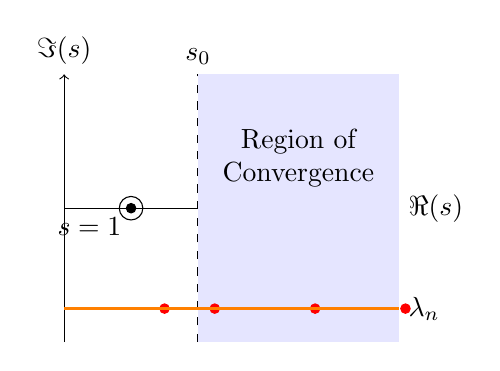
\begin{tikzpicture}[scale=0.85]
    % Draw a visualization of the spectral zeta function
    % Draw axes
    \draw[->] (0,0) -- (5,0) node[right] {$\Re(s)$};
    \draw[->] (0,-2) -- (0,2) node[above] {$\Im(s)$};
    
    % Draw region of convergence
    \draw[dashed] (2,-2) -- (2,2);
    \node[above] at (2,2) {$s_0$};
    \fill[blue!10] (2,-2) rectangle (5,2);
    \node at (3.5,1) {Region of};
    \node at (3.5,0.5) {Convergence};
    
    % Draw some illustrative zeros/poles
    \filldraw (1,0) circle (2pt);
    \node[below left] at (1,0) {$s=1$};
    \draw (1,0) circle (5pt);
    
    % Draw some eigenvalues on the spectrum
    \foreach \x in {0.5, 0.75, 1.25, 1.7} {
        \filldraw[red] (\x*3, -1.5) circle (2pt);
    }
    \draw[thick, orange] (0,-1.5) -- (5,-1.5);
    \node[right] at (5,-1.5) {$\lambda_n$};
\end{tikzpicture}
\caption{A visualization of the operator-valued zeta function showing the region of convergence and the relationship to the eigenvalue spectrum.}
\label{fig:spectral_zeta}
\end{figure}